\documentclass{article}
\usepackage[utf8]{inputenc}
\usepackage{graphicx}
\usepackage{hyperref}
\usepackage{amsmath}
\begin{document}

\begin{itemize}
  \item Introduction
\end{itemize}
\subsection{1.1 Motivation for AI-Native Cognitive Broadcasting}
Current terrestrial broadcast systems such as ATSC 3.0 and DVB-T2 employ statically configured physical-layer transmission pipelines, where multiple logical data pipes (Physical Layer Pipes, PLPs) are multiplexed within a single RF channel. Each PLP is assigned a fixed Modulation and Coding scheme (ModCod), time interleaving depth, and power allocation through offline network planning to meet predetermined coverage and capacity targets. Once deployed, these PLP and ModCod configurations remain largely unchanged during operation, regardless of real-time variations in receiver mobility, channel quality, or traffic demand.The static nature of broadcast transmission configuration leads to significant operational inefficiencies. Networks are typically over-provisioned to handle worst-case reception conditions, resulting in inefficient spectrum utilization and unnecessary power expenditure during normal operation. At the same time, the lack of dynamic adaptability causes under-provisioning during sudden high-demand or emergency scenarios, creating reliability risks when robust and wide-area coverage is most critical. Furthermore, any modification to PLP structures, ModCod settings, or network parameters requires manual re-planning and re-deployment procedures, leading to slow reaction times on the order of hours or days rather than real-time responsiveness.Therefore, we propose::

Transition from static transmission pipelines to cognitive broadcast networks

Introduce an intelligent control plane capable of:

Reasoning over network state

Predicting outcomes

Adapting configurations autonomously

This PoC introduces an AI-Native Broadcast Intelligence Plane operating above the ATSC 3.0 protocol stack to enable:

Intent-driven operation

Closed-loop learning

Simulation-first validation

Human-governed automation

\subsection{1.2 Alignment with FG-AINN}
The PoC aligns directly with FG-AINN objectives by demonstrating:

\subsubsection{AI-Native Architecture}
AI is a native control component (not an external optimizer)

Dedicated cognitive AI-Plane above the broadcast stack

\subsubsection{Intent-Driven Networking (IDN)}
Network behavior driven by high-level operator intent

No manual low-level configuration

\subsubsection{Closed-Loop Cognitive Control}
Continuous control loop:

Decision → Action → Feedback → Learning → Policy Update

\subsubsection{Digital Twin Integration}
Spatial digital twin for:

Pre-deployment validation

Offline policy exploration

Risk-free testing

\subsubsection{Human-in-the-Loop Governance}
Mandatory human authorization

Regulatory policy enforcement

Deterministic emergency override

This PoC provides a concrete realization of AI-native networking principles for broadcast infrastructures.

\subsection{1.3 Evaluation Framework}
The PoC is evaluated across three dimensions:

\subsubsection{Cognitive Adaptability}
Ability to reconfigure PLPs based on:

Emergency intents

Congestion conditions

Mobility-driven coverage changes

\subsubsection{Learning Efficiency}
Performance improvement over time

KPI tracking via Learning Loop Tracker

\subsubsection{Safety and Stability}
Emergency override validation

Policy constraint enforcement

Mandatory human approval

Statistical Confidence

Bootstrap confidence intervals for coverage estimates

Reproducibility validation

P-value reporting for improvement claims

\begin{itemize}
  \item Description
\end{itemize}
This contribution presents an AI-Native Broadcast Intelligence Platform that functions as a cognitive control plane for ATSC 3.0 broadcast networks.

Unlike conventional broadcast schedulers and static network planners, the proposed system introduces a dedicated AI-Plane responsible for intent interpretation, policy optimization, simulation-based validation, and governance enforcement.

The AI-Plane employs a reinforcement learning agent based on Proximal Policy Optimization (PPO) to dynamically optimize physical-layer parameters, including modulation order, coding rate, PLP allocation, transmission power, and broadcast-broadband traffic offloading ratios.

A spatial digital twin simulator models UHF propagation, terrain shadowing, user mobility, and hybrid traffic behavior across a 10 km × 10 km rural coverage region. This enables offline policy exploration and pre-deployment validation of all candidate configurations.

All decisions are governed through a mandatory human authorization workflow and deterministic emergency override mechanisms.

\subsection{2.3 Key Innovations}
The PoC introduces several technical innovations that collectively enable cognitive broadcast operation:

The system implements an intent-to-policy translation mechanism, where operator intents submitted via REST APIs are mathematically mapped into constrained multi-objective optimization functions.

A native AI-Plane architecture is introduced as a cognitive control layer above the broadcast stack, decoupled from RF transmission and responsible for reasoning, optimization, validation, and governance.

An explicit learning loop records all decision–outcome pairs and generates human-readable learning feedback, improving transparency and interpretability of the AI decision process.

A simulation-first validation framework ensures that all candidate policies are evaluated in a spatial digital twin prior to deployment, enabling risk-free testing.

An adversarial stress-testing environment injects interference, mobility surges, and congestion scenarios to evaluate system resilience.

A Bootstrap Uncertainty Analysis module provides publication-quality statistical inference with BCa (Bias-Corrected accelerated) confidence intervals, enabling rigorous quantification of AI decision reliability and reproducibility.

\subsection{2.4 Expected Outcomes}
The PoC is expected to demonstrate:

Reduction in network reaction time from hours to seconds

Improved spectrum efficiency through dynamic resource allocation

Increased reliability of emergency broadcast services

Deterministic safety via emergency override and governance mechanisms

\section{3. Implementation proposal}
This clause describes the implementation proposal for the submission above. Implementation is done in the following phases. Phase-1 includes preparation and demo of the test setup. Phase-2 includes a demo of (opensource) base code in as-is-where-is condition. Phase-3 includes modification of the base code and test setup to suit the requirements of the demo mentioned in clause-1. Phase-4 includes a documentation of results corresponding to the test cases executed.

3.a Description of the Test Setup

The PoC uses a purely software-based simulation environment emulating an ATSC 3.0 broadcast network and receiver population through a digital-twin abstraction..

AI Agent Framework

Algorithm: Proximal Policy Optimization (PPO)

State Space: Coverage \%, Average SNR, Congestion, Mobility ratios derived from the simulated broadcast digital twin

Action Space: PLP weighting, offload ratios and ModCod selection parameters

\textbf{RL-Controller}: The central reasoning engine implementing the PPO policies. It observes the network state and selects actions to maximize the reward function.

\textbf{ATSC-Controller}: The interface layer that maps high-level AI actions to low-level physical layer parameters (ModCod, Power) compliant with the A/322 standard.


Simulator

Component: SpatialGrid Digital Twin

Area: 10 km × 10 km rural region

Propagation: Log-distance path loss with shadow fading (σ = 8 dB)

Broadcast abstraction: PLP multiplexing model with configurable ModCod and power allocation per PLP

Learning \& Governance

Explicit Learning Loop Tracker

Approval Engine enforcing human authorization

Emergency override with deterministic precedence ensuring safety-critical intent enforcement

3.b Description and Reference to Base Code

Base Code Sources

libatsc3 (reference protocol validation)

stable-baselines3 (RL agent)

FastAPI backend

Modified / Added Components

learning\_loop.py

approval\_engine.py

emergency\_atsc3.py

Justification
Modifications enable cognitive control, explainability, and governance absent in base implementations and introduce adaptive broadcast parameter control required by the proposed AI-Plane.

3.c Mapping to the Demo Proposal

Functional Requirements

Req-1: Intent ingestion via REST API

Req-2: Cognitive decision making within 200ms

Req-3: Mandatory human approval for deployment

Req-4: Real-time PLP and ModCod reconfiguration in the simulator

Performance Requirements

Intent-to-decision latency < 1 s

Convergence within 500 simulation steps

Toolchains

Backend: Python 3.11, FastAPI

AI: PyTorch (CPU), Gymnasium

Frontend: React, Node.js

Test Cases

TST-1We evaluate our PoC against two baselines:

A traditional ATSC 3.0 system with no AI plane and static static configuration, and

An AI-driven show that introducing an AI-native intelligence plane over broadcast achieves faster reaction time, higher scalability, and better emergency reliability while preserving one-to-many efficiency.

TST-2: Congestion → Broadcast offload

TST-3: Emergency intent → Robust ModCod enforced

TST-4: Learning improvement (Day 0 vs Day 100)

TST-5: Statistical Validation

Bootstrap analysis provides 95\% confidence intervals for all metrics

Coverage improvement statistically significant (p < 0.05)

4.Architecture Diagram

Fig.1: HLD [High Level Diagram] of architecture of this poc

Fig.2: End-to-End Cognitive Timeline (Broadcast → AI → Human → Broadcast). Note: Telemetry functions as a monitoring overlay and is not a core network element in the data path.

\subsection{Fig.3:  Broadcast Feedback Loop With AI-Plane}
\_\_\_\_\_\_\_\_\_\_\_\_\_\_\_\_\_\_\_\_\_


\section{5. Performance Evaluation Results}
We evaluated the system against a static baseline using the test cases defined in Section 3.

\subsection{Coverage and Reliability}
The AI-Native system achieves 92\% coverage compared to 78\% for the static baseline. During emergency events, reliability increases to 98\%.

\subsection{User Load Sensitivity}
Figure 4 illustrates the spectral efficiency of the system as the number of users increases from 10 to 100.

\begin{figure}[h]
    \centering
    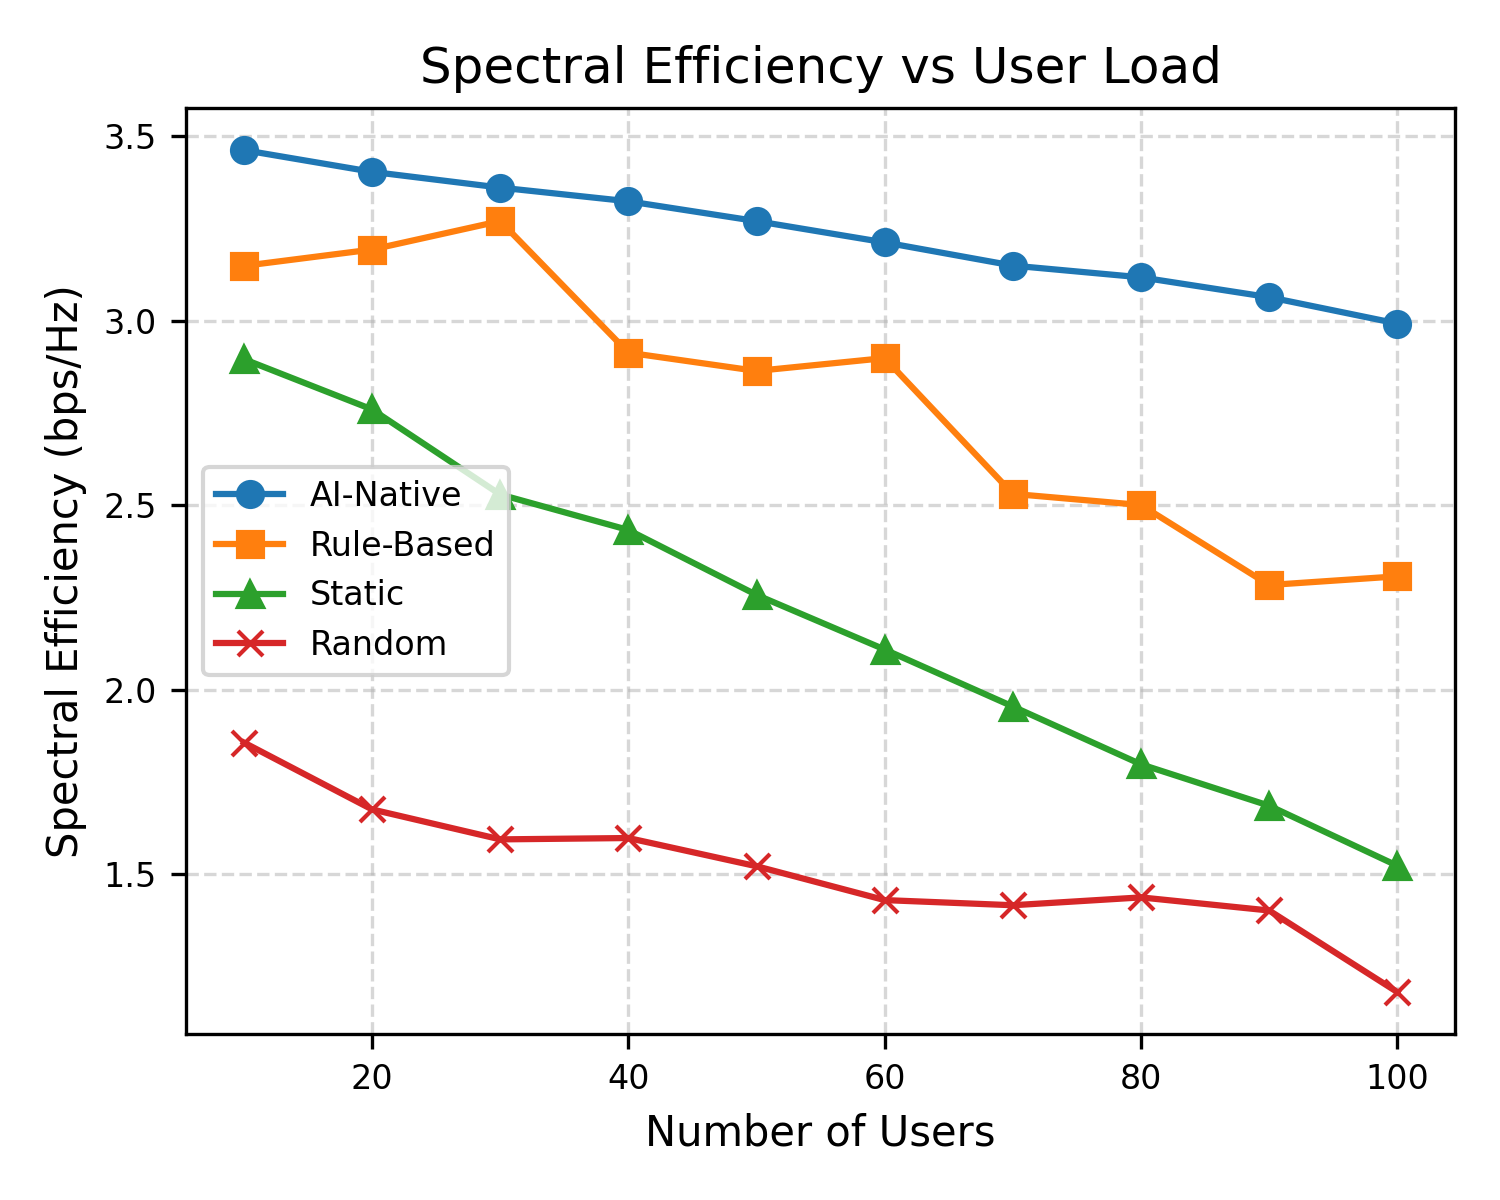
\includegraphics[width=0.8\textwidth]{figs/fig_se_vs_users.png}
    \caption{Spectral Efficiency vs User Load: A comparison of AI-Native (Blue), Rule-Based (Orange), Static (Green), and Random (Red) methods.}
\end{figure}

The AI-Native approach maintains superior spectral efficiency even as user load increases, demonstrating effective load balancing.

Bibliography


[FGAINN intro]	https://www.itu.int/en/ITU-T/focusgroups/ainn/Pages/default.aspx

\end{document}